\section{Moto rettilineo smorzato esponenzialmente}
\label{section:MRSE}
%---------------------------------------------------------------------------
Questo tipo di moto si incontra quando si ha un'accelerazione proporzionale
alla velocità con coefficiente negativo (altrimenti sarebbe forzato esponenzialmente nel tempo). Introduciamo quindi un parametro di smorzamento $\beta>0$.
\begin{equation*}
    a_{(t)} = -\beta v_{(t)} = \dot v_{(t)}\seg \frac{\dot v}{v} =
    -\beta \seg \int_{t_0}^{t}dt' \frac{\dot v}{v} =  -\beta\int_{t_0}^{t}dt'\seg
\end{equation*}
\begin{equation}
    \seg\ln{\left[ \frac{v_{(t)}}{v_0}\right]} =
    -\beta\sx t-t_0\dx\seg \boxed{v_{(t)} = v_0e^{-\beta\sx t-t_0\dx}} = \dot x 
\end{equation}
\begin{equation}
    \boxed{x_{(t)} = x_0 + \frac{v_0}\beta\left[1-e^{-\beta\sx t-t_0\dx}\right]}
\label{eq:MRSE}
\end{equation}
\begin{equation}
    a = -\beta \cancel{v} = \cancel{v}\frac{dv}{dx}\seg
    \boxed{v_{(x)} = v_0 - \beta\sx x - x_0\dx}
\label{eq:v(x)_MRSE}
\end{equation}

\begin{figure}[htbp]
    \begin{center}
        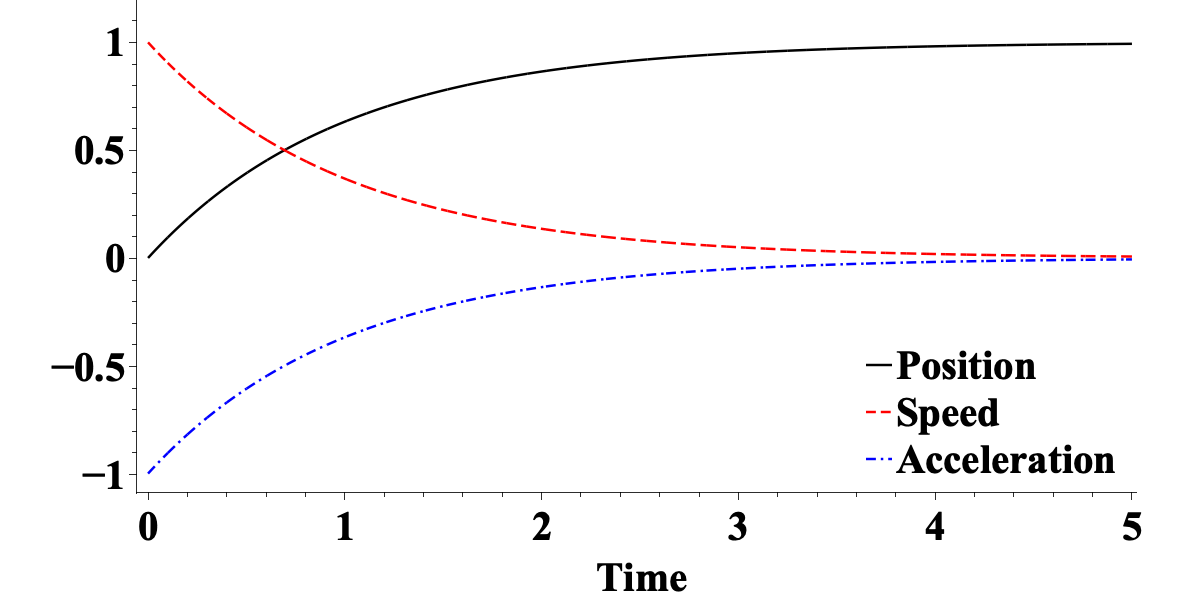
\includegraphics[width=13cm]{images/MRSE.png} 
        \caption{Un esempio del grafico di accelerazione (rosso), velocità (verde)
        e posizione (blu), nel moto smorzato esponenzialmente. L'asse delle
        ascisse rappresenta il tempo, mentre quello delle ordinate
        la variabile dipendente.}
    \end{center}
\label{fig:MRSE}
\end{figure}